   %% LyX 2.3.4.2 created this file.  For more info, see http://www.lyx.org/.
%% Do not edit unless you really know what you are doing.
\documentclass[11pt,oneside,american,czech]{book}
\usepackage[T1]{fontenc}
\usepackage[utf8]{inputenc}
\usepackage[a4paper]{geometry}
\geometry{verbose,tmargin=4cm,bmargin=3cm,lmargin=3cm,rmargin=2cm,headheight=0.8cm,headsep=1cm,footskip=0.5cm}
\pagestyle{headings}
\setcounter{secnumdepth}{3}
\usepackage{url}
\usepackage{amsmath}
\usepackage{amsthm}
\usepackage{amssymb}
\usepackage{graphicx}
\usepackage{setspace}
\usepackage{hyperref}
\usepackage{libertine}
\usepackage{comment}
\usepackage{calrsfs}
\makeatletter
%%%%%%%%%%%%%%%%%%%%%%%%%%%%%% Textclass specific LaTeX commands.
\newenvironment{lyxlist}[1]
	{\begin{list}{}
		{\settowidth{\labelwidth}{#1}
		 \setlength{\leftmargin}{\labelwidth}
		 \addtolength{\leftmargin}{\labelsep}
		 \renewcommand{\makelabel}[1]{##1\hfil}}}
	{\end{list}}

%%%%%%%%%%%%%%%%%%%%%%%%%%%%%% User specified LaTeX commands.
%% Font setup: please leave the LyX font settings all set to 'default'
%% if you want to use any of these packages:

%% Use Times New Roman font for text and Belleek font for math
%% Please make sure that the 'esint' package is turned off in the
%% 'Math options' page.
\usepackage[varg]{txfonts}

%% Use Utopia text with Fourier-GUTenberg math
%\usepackage{fourier}

%% Bitstream Charter text with Math Design math
%\usepackage[charter]{mathdesign}

%%---------------------------------------------------------------------

%% Make the multiline figure/table captions indent so that the second
%% line "hangs" right below the first one.
%\usepackage[format=hang]{caption}

%% Indent even the first paragraph in each section
\usepackage{indentfirst}

%%---------------------------------------------------------------------

%% Disable page numbers in the TOC. LOF, LOT (TOC automatically
%% adds \thispagestyle{chapter} if not overriden
%\addtocontents{toc}{\protect\thispagestyle{empty}}
%\addtocontents{lof}{\protect\thispagestyle{empty}}
%\addtocontents{lot}{\protect\thispagestyle{empty}}

%% Shifts the top line of the TOC (not the title) 1cm upwards 
%% so that the whole TOC fits on 1 page. Additional page size
%% adjustment is performed at the point where the TOC
%% is inserted.
%\addtocontents{toc}{\protect\vspace{-1cm}}

%%---------------------------------------------------------------------

% completely avoid orphans (first lines of a new paragraph on the bottom of a page)
\clubpenalty=9500

% completely avoid widows (last lines of paragraph on a new page)
\widowpenalty=9500

% disable hyphenation of acronyms
\hyphenation{CDFA HARDI HiPPIES IKEM InterTrack MEGIDDO MIMD MPFA DICOM ASCLEPIOS MedInria}

%%---------------------------------------------------------------------

%% Print out all vectors in bold type instead of printing an arrow above them
\renewcommand{\vec}[1]{\boldsymbol{#1}}
\newcommand{\R}{\mathbb{R}}
\newtheorem{definition}{Definice}[section]
\newtheorem{vet}{Věta}[section]
\newtheorem*{poz}{Poznámka}
\newtheorem*{pří}{Příklad}
\newcommand{\N}{\mathbb{N}}
\newcommand{\C}{\mathbb{C}}
\newcommand{\Z}{\mathbb{Z}}
%  Matematika
\newcommand{\ee}{\mathrm{e}} %eulerovo číslo
\newcommand{\ii}{\mathrm{i}} %imaginární jednotka
\newcommand{\inR}{\in \mathbb{R}}
\newcommand{\dd}{\mathrm{d}}
\newcommand\KLDeq{\mathrel{\stackrel{\makebox[0pt]{\mbox{\normalfont\tiny KLD}}}{\approx}}}
\newcommand*{\matr}[1]{\mathbfit{#1}}
\newcommand*{\tran}{^{\mkern-1.5mu\mathsf{T}}}
\newcommand*{\conj}[1]{\overline{#1}}
\newcommand*{\hermconj}{^{\mathsf{H}}}
\DeclareMathOperator{\tr}{tr}
\DeclareMathOperator*{\argmin}{arg\,min} 
\DeclareMathAlphabet{\pazocal}{OMS}{zplm}{m}{n}
% Jednotky
\newcommand{\unit}[1]{\,\mathrm{#1}} %jednotky zadávejte pomocí tohoto příkazu
\renewcommand{\deg}{\ensuremath{\mathring{\;}}} %symbol stupně
\newcommand{\celsius}{\ensuremath{\deg\mathrm{C}}} %stupně celsia

%(hodnota plus mínus chyba) jednotka
\newcommand{\hodn}[3]{(#1 \pm #2)\unit{#3}} 

%veličina [jednotka] do hlavičky tabulky
\newcommand{\tabh}[2]{\ensuremath{#1\,[\mathrm{#2}]}} 
% Replace standard \cite by the parenthetical variant \citep
%\renewcommand{\cite}{\citep}
\newcommand{\diag}{\mathop{\mathrm{diag}}}
\def\Var{{\textrm{Var}}\,}



\makeatother

\usepackage{babel}
\begin{document}
\def\documentdate{7. \v{c}ervence 2020}

%%\def\documentdate{\today}

\pagestyle{empty}
{\centering

\noindent %
\begin{minipage}[c]{3cm}%
\noindent \begin{center}

\includegraphics[width=3cm,height=3cm,keepaspectratio]{Images/TITLE/cvut}
\par\end{center}%
\end{minipage}%
\begin{minipage}[c]{0.6\linewidth}%
\begin{center}
\textsc{\large{}České vysoké učení technické v Praze}{\large{}}\\
{\large{}Fakulta jaderná a fyzikálně inženýrská}
\par\end{center}%
\end{minipage}%
\begin{minipage}[c]{3cm}%
\noindent \begin{center}

\includegraphics[width=3cm,height=3cm,keepaspectratio]{Images/TITLE/fjfi}
\par\end{center}%
\end{minipage}

\vspace{3cm}

\textbf{\huge{}Generativní modely dat popsaných stromovou strukturou}{\huge\par}

\vspace{1cm}

\selectlanguage{american}%
\textbf{\huge{}Generative models of tree structured data}{\huge\par}

\selectlanguage{czech}%
\vspace{2cm}

{\large{}Bakalářská práce}{\large\par}

}

\vfill{}

\begin{lyxlist}{MMMMMMMMM}
\begin{singlespace}
\item [{Autor:}] \textbf{Jakub Bureš}
\item [{Vedoucí~práce:}] \textbf{Doc. Ing. Václav Šmídl, Ph.D.}
\item [{Konzultant:}] \textbf{Doc. Ing. Tomáš Pevný, Ph.D.}
\item [{Akademický~rok:}] 2019/2020
\end{singlespace}
\end{lyxlist}
\newpage{}

~

\vfill{}

\begin{center}
\begin{enumerate}	
\item Seznamte se s popisem dat pomocí stromové struktury. Zvláštní pozornost věnujte metodám více instančního učení (multiple instance learning). Seznamte se s konceptem vnořeného prostoru (embedded space) a jeho reprezentace pomocí neuronových sítí. 
\item	
Seznamte se se základními generativními modely dat popsaných vektorem příznaků. Zvláštní pozornost věnujte metodám typu autoencoder a jejich variační formě. Demonstrujte vlastnosti modelů na jednoduchých příkladech. V maximální míře využijte dostupné knihovny pro generativní modely.
\item
Navrhněte několik příkladů typů dat se stromovou strukturou a pro každý z nich navrhněte generativní model. Navrhněte algoritmus pro určení jeho parametrů z dat a diskutujte vhodnost jednotlivých architektur neuronových sítí.
\item
Seznamte se s různými druhy apriorních rozložení používaných na latentní proměnné autoencoderu. Odvoďte algoritmy odhadu jejich parametrů a srovnejte jejich výsledky se základním modelem. Diskutujte výsledné odhady.
\item	
Vyvinutou metodu aplikujte na vhodně zvolená reálná data a diskutujte vliv zvoleného apriorního rozložení na výsledky.
\end{enumerate}
\par\end{center}

\vfill{}

~\newpage{}

~

\vfill{}

\begin{center}
- Zadání práce (zadní strana) -
\par\end{center}

\vfill{}

~\newpage{}

\noindent \emph{\Large{}Poděkování:}{\Large\par}

\noindent Chtěl bych zde poděkovat především svému školiteli panu Doc. Ing. Václavu Šmídlovi, Ph.D.
za pečlivost, ochotu, vstřícnost a odborné i lidské zázemí při vedení
mé bakalářské práce. Dále děkuji svému konzultantovi panu Doc. Ing. Tomáši Pevnému, Ph.D.

\vfill

\noindent \emph{\Large{}Čestné prohlášení:}{\Large\par}

\noindent Prohlašuji, že jsem tuto práci vypracoval samostatně a uvedl
jsem všechnu použitou literaturu.

\bigskip{}

\noindent V Praze dne \documentdate\hfill{}Jakub Bureš

\vspace{2cm}

\newpage{}

\begin{onehalfspace}
\noindent \emph{Název práce:} 

\noindent \textbf{Generativní modely dat popsaných stromovou strukturou}
\end{onehalfspace}

\bigskip{}

\noindent \emph{Autor:} Jakub Bureš

\bigskip{}

\noindent \emph{Obor:} Matematické inženýrství
 \bigskip{}

\noindent \emph{Zaměření:} Aplikované matematicko-stochastické metody

\bigskip{}

\noindent \emph{Druh práce:} Bakalářská práce

\bigskip{}

\noindent \emph{Vedoucí práce:} Doc. Ing. Václav Šmídl, Ph.D.\\
ÚTIA AV ČR
Pod vodárenskou věží 4
182 00 Praha 8

\bigskip{}

\noindent \emph{Konzultant:} Doc. Ing. Tomáš Pevný, Ph.D. \\
Katedra počítačů
FEL ČVUT Praha
Technická 1902/2
166 27 Praha 6 - Dejvice
\bigskip{}

\noindent \emph{Abstrakt:} Abstrakt max. na 10 řádků. Abstrakt max.
na 10 řádků. Abstrakt max. na 10 řádků. Abstrakt max. na 10 řádků.
Abstrakt max. na 10 řádků. Abstrakt max. na 10 řádků. Abstrakt max.
na 10 řádků. Abstrakt max. na 10 řádků. Abstrakt max. na 10 řádků.
Abstrakt max. na 10 řádků. Abstrakt max. na 10 řádků. Abstrakt max.
na 10 řádků. Abstrakt max. na 10 řádků. Abstrakt max. na 10 řádků.
Abstrakt max. na 10 řádků. Abstrakt max. na 10 řádků. Abstrakt max.
na 10 řádků. Abstrakt max. na 10 řádků. Abstrakt max. na 10 řádků.
Abstrakt max. na 10 řádků. Abstrakt max. na 10 řádků. Abstrakt max.
na 10 řádků. Abstrakt max. na 10 řádků. Abstrakt max. na 10 řádků.
Abstrakt max. na 10 řádků. Abstrakt max. na 10 řádků. Abstrakt max.
na 10 řádků. Abstrakt max. na 10 řádků. Abstrakt max. na 10 řádků. 

\bigskip{}

\noindent \emph{Klíčová slova:} klíčová slova (nebo výrazy) seřazená
podle abecedy a oddělená čárkou

\vfill{}
~

\selectlanguage{american}%
\begin{onehalfspace}
\noindent \emph{Title:}Generative models of tree structured data 

\noindent \textbf{Generative models of tree structured data}
\end{onehalfspace}

\bigskip{}

\noindent \emph{Author:} Jakub Bureš

\bigskip{}

\noindent \emph{Abstract:} Max. 10 lines of English abstract text.
Max. 10 lines of English abstract text. Max. 10 lines of English abstract
text. Max. 10 lines of English abstract text. Max. 10 lines of English
abstract text. Max. 10 lines of English abstract text. Max. 10 lines
of English abstract text. Max. 10 lines of English abstract text.
Max. 10 lines of English abstract text. Max. 10 lines of English abstract
text. Max. 10 lines of English abstract text. Max. 10 lines of English
abstract text. Max. 10 lines of English abstract text. Max. 10 lines
of English abstract text. Max. 10 lines of English abstract text.
Max. 10 lines of English abstract text. Max. 10 lines of English abstract
text. Max. 10 lines of English abstract text. Max. 10 lines of English
abstract text. Max. 10 lines of English abstract text. Max. 10 lines
of English abstract text. Max. 10 lines of English abstract text.
Max. 10 lines of English abstract text. Max. 10 lines of English abstract
text. Max. 10 lines of English abstract text.

\bigskip{}

\noindent \emph{Key words:} keywords in alphabetical order separated
by commas

\selectlanguage{czech}%
\newpage{}

\pagestyle{plain}

\tableofcontents{}

\newpage{}




\chapter*{Úvod}

\chapter{Teorie}
\section{Optimalizace}
Optimalizace je matematická úloha, jejíž snahou je nalezení takových hodnot proměnných, pro které daná funkce nabývá minima či maxima. My se budeme snažit najít minimální hodnoty parametrů $\theta$ tzv. ztrátové funkce, kterou budeme značit $L(\theta)$ z anglického výrazu loss function. 
Minimalizací ztrátové funkce získáme 
\begin{equation}\label{argminL}
\hat{\theta} = \argmin_{\theta} L(\theta)
\end{equation}
Existuje nespočet způsobů jak danou funkci minimalizovat. My budeme výhradně používat metodu zvanou Gradient Descent.

\subsection{Gradient Descent}
Jedná se iterativní optimalizační metodu. 
  Minimalizujeme $L(\theta)$, tedy derivujeme dle vektoru parametrů $\theta$, díky čemuž dostaneme $\nabla_{\theta}\ L(\theta) $. Symbol $\nabla_{\theta}$ značí gradient funkce $L(\theta)$ přes všechny hodnoty $\theta$.
Použijeme bod $\theta_0$ funkce $L(\theta)$ jako výchozí bod, ze kterého se pohybujeme ve směru záporného gradientu s krokem $h$~$\in$~$\mathbb{R}_{+}$.  Matematickou interpretaci toho postupu můžeme vyjádřit následujícím zápisem:
\begin{equation}\label{GradientDescent}
\theta_{n+1} = \theta_{n} - h\cdot \nabla_{\theta} L(\theta_n)
\end{equation}
 Tento postup provádíme, dokud nejsme v minimu funkce a získáme tak vektor parametrů $\hat{\theta}$, jak je popsáno v \eqref{argminL}.
\subsection*{ADAM}
Předchozí metoda není při větším množství dat tak rychlá, jak bychom pro výpočet minima ztrátové funkce potřebovali. Používáme proto adaptivní iterační gradientní metodu ADAM (Adaptive Moment Estimation), která navíc používá druhý moment gradientu. Zatímco Gradient descent má krok stále stejný, u metody ADAM je krok $h$ adaptivní. Popřípadě můžeme ladit i zapomínací koeficienty, což už je ale mimo rámec této práce a my nebudeme při výpočtech využívat.
\pagestyle{headings}
\subsection{Metoda nejmenších čtverců}\label{least_squares}
 Předpokládejme že máme množinu $x = \left \lbrace x_{i}\right\rbrace_{i = 1}^{n} $ ke každému $x_i$ máme právě jedno pozorování $y_i$, komplexně zapsáno zobrazením jako $(x_1,\dots, x_n)~\longmapsto~(y_1,\dots, y_n)$.
Naším cílem je najít nejlepší proložení dat, čili fit, pomocí polynomické funkce řádu $p\leq n$ ve tvaru
\begin{equation}\label{linear_combination}
\hat{y}(x, \theta) = \theta_0 + \theta_1x + \theta_2x^2 + \dots + \theta_px^p = \sum_{i = 0}^{p} {\theta_{i}x^{i}},
\end{equation}
která je lineární v neznámých parametrech $\theta = \left( \theta_0, \theta_1,\dots, \theta_p\right)$. Takové modely nazýváme lineární a jednoduše je nazýváme lineární regresí. Jelikož se jedná o tak jednoduché modely, jejich míra využití je značně omezena. O tom jak tyto modely vylepšit, se dozvíme v kapitole \eqref{generative}. \\
Abychom našli ten nejlepší možný fit, je nutno minimalizovat ztrátovou funkci $L(\theta)$:  
\begin{equation}\label{eq:loss}
L(\theta) =\sum_{i = 1}^{n}\left[ \hat{y}(x_i, \theta) - y_i\right]^2 = \left( \mathbb{X}\cdot\theta - y \right)\tran\left(  \mathbb{X}\cdot\theta - y \right)
\end{equation}
Tato funkce znázorňuje čtverec vzdálenosti pozorovaní $y$ k hledané funkci $\hat{y}(x, \theta)$, jenž chceme mít co nejmenší - proto metoda nejmenších čtverců.
Matice $\mathbb{X}$ je tvaru
\begin{equation}
\mathbb{X} =
\begin{pmatrix}
1 & x_1 & x_1^2 & \dots & x_1^p \\
1 & x_2 & x_2^2 & \dots & x_2^p \\
\vdots & \vdots &\vdots & \ddots &\vdots\\
1 & x_n & x_n^2 & \dots & x_n^p \\
\end{pmatrix}
\end{equation}


Odhadovat parametry $\theta$ můžeme pomocí gradientní metody a to způsobem, který je popsán rovnicí \eqref{GradientDescent}. Najdeme gradient ztrátové funkce
\begin{equation}
\nabla_{\theta}\ L(\theta) = 2\mathbb{X}\tran(\mathbb{X}\cdot\theta - y)
\end{equation}
a postupujeme pomocí \eqref{GradientDescent}, dokud nezískáme $\hat{\theta} = \argmin_{\theta} L(\theta)$. \\
Metoda nejmenších čtverců má ovšem analytické řešení. Systém rovnic můžeme zapsat formou matice a vektorů 
\begin{equation*}
\begin{pmatrix}
y_1 \\
y_2\\
\vdots \\
y_n
\end{pmatrix}
=
\begin{pmatrix}
1 & x_1 & x_1^2 & \dots & x_1^p \\
1 & x_2 & x_2^2 & \dots & x_2^p \\
\vdots & \vdots &\vdots & \ddots &\vdots\\
1 & x_n & x_n^2 & \dots & x_n^p \\
\end{pmatrix}
\cdot
\begin{pmatrix}
\theta_0 \\
\theta_1 \\
\vdots \\
\theta_p
\end{pmatrix}
+
\begin{pmatrix}
\varepsilon_0 \\
\varepsilon_1 \\
\vdots \\
\varepsilon_p
\end{pmatrix}
\end{equation*}
 Pro jednoduchost budeme tímto zápisem rozumět následující rovnici
\begin{equation}\label{eq:regresematrix}
y = \mathbb{X} \cdot {\theta} + \epsilon
\end{equation}
Naším cílem je získání parametrů $\theta$. Jelikož je $y - \hat{y}= \epsilon $, přepíšeme rovnici pomocí $\hat{y}$, čímž získáme
\begin{equation}\label{eq:regresematrix}
\hat{y} = \mathbb{X} \cdot {\theta} 
\end{equation}
 a obě strany rovnice vynásobíme zleva $ \mathbb{X}\tran$. Tím nám rovnice přejde do tvaru
\begin{equation*}
\mathbb{X}\tran\cdot \hat{y} = \mathbb{X}\tran\cdot \mathbb{X} \cdot {\theta}
\end{equation*}
Teď už stačí rovnici zleva vynásobit inverzní maticí $(\mathbb{X}\tran\cdot \mathbb{X})^{-1}$. Dostaneme tak konečné řešení
\begin{equation}\label{regresethetahat}
\hat{\theta} = (\mathbb{X}\tran \mathbb{X})^{-1}\mathbb{X}\tran \hat{y}
\end{equation}
Tento postup zahrnuje i lineární regresi pro hodnotu $p = 1$.

\newpage

\section{Úvod do pravděpodobnosti a Bayesovská statistika}
\subsection{Pravděpodobnostní míra}
\begin{definition}[Kolmogorova definice pravděpodobnosti]
Mějme množinu $\Omega$ vybavenou $\sigma$-algebrou $\mathcal{A}$, tedy souborem podmnožin obsahujícím $\Omega$ a uzavřeným na doplňky a spočetná sjednocení. Pak libovolnou funkci $P : \mathcal{A} \to \mathbb{R}$ , která splňuje :
\begin{enumerate}
\item $(\forall A\in \mathcal{A})(P(A) \geq 0).$
\item$ P(\Omega) = 1 $
\item $\forall A_j $ disjunktní platí $P(\sum_{j=1}^{\infty}A_j) = \sum_{j=1}^{\infty}P(A_j)$
\end{enumerate}
nazýváme pravděpodobnostní mírou.
\end{definition}
\begin{vet}[Vlastnosti $P$] Mějme pravděpodobnostní prostor $(\Omega,\mathcal{A}, P)$ a nechť $(\forall j \in \mathbb{N})(A_j \in \mathcal{A})$ a $B \in \mathcal{A}$. Pak platí:
\begin{enumerate}


\item $P(\emptyset) = 0$,
\item Aditivita:  $P(\sum_{j=1}^{n}A_j) = \sum_{j=1}^{n}P(A_j)$,
\item Monotonie: $A\subset B \Rightarrow P(A) \leq P(B)$,
\item Subtraktivita: $A\subset B \Rightarrow P(B\smallsetminus A) = P(B) - P(A)$,
\item Omezenost: $(\forall A \in \mathcal{A})(P(A)\leqslant 1) $,
\item Komplementarita: $A \in \mathcal{A} \Rightarrow P(A^C) = 1 - P(A)$
\end{enumerate}
\end{vet}
\begin{definition}[Podmíněná pravděpodobnost] Nechť $A,B \in \mathcal{A}$ a $P(B)>0$. Pak definujeme podmíněnou pravděpodobnost:
\begin{equation}\label{podminenapravdepodobnost}
P(A|B) = \frac{P(A,B)}{P(B)}
\end{equation}

\end{definition}
\begin{vet}[Součinové pravidlo]
Nechť $A_1,\ldots,A_n \in \mathcal{A} $ a dále nechť také $P(A_1,\ldots,A_n ) > 0$. Potom platí:
\begin{equation}\label{chainrule}
P(A_1,\ldots,A_n) = P(A_1)\cdot P(A_2|A_1) \cdot P(A_3| A_2, A_1)\cdot \ldots \cdot P(A_n|A_1,\ldots,A_{n-1})
\end{equation}
\end{vet}
\begin{vet}[Bayesova věta] Nechť $A \in \mathcal{A} $ a $P(B) \neq 0$. Potom platí:
\begin{equation}\label{Bayes}
P(A|B) = \frac{P(B\vert A)P(A)}{P(B)}
\end{equation}
\end{vet}
$P(A)$ nazýváme prior a $P(A|B)$ nazýváme posterior.

\begin{vet}[Nezávislost jevů] Nechť $A_j \in \mathcal{A} (\forall j \in \mathbb{N})$. Potom jevy nazveme nezávislé právě tehdy když platí podmínka
\begin{equation}
P(A_1,\ldots,A_k) = \prod_{i=1}^{k} P(A_i)
\end{equation}
\end{vet}

\subsection{Hustoty pravděpodobnosti}
Primárním cílem generativního modelování je hledání distribuce nebo-li hustoty pravděpodobnosti daných dat. Výhodou je, že pro hustotu pravděpodobnosti můžeme využívat stejně pravidlo podmíněnosti \eqref{podminenapravdepodobnost}, součinové pravidlo \eqref{chainrule} a Bayeseovo pravidlo \eqref{Bayes}. Toto se pro nás ukáže jako naprosto klíčové. 
\begin{definition}[Náhodná veličina]
Máme prostor $\left(\Omega,\mathcal{A} \right)$, potom funkci $\textbf{X} = \left(X_1,\dots,X_n \right):(\Omega,\mathcal{A})\rightarrow \left(\R^n,\mathcal{B}_n \right)$, kde $\mathcal{B}_n $ značí borelovskou $\sigma$-algrebru v $\R^n$, nazveme náhodnou veličinou.
\end{definition}
\begin{definition}[Hustota pravděpodobnosti]
\label{hustota}
Hustotou pravděpodobnosti náhodné veličiny $\textbf{X}$ rozumíme spojitou funkci $p_{\textbf{X}}\left(\textbf{x}\right)$, která splňuje následující dvě podmínky:
\begin{enumerate}
\item $\forall \textbf{x}$, $p_{\textbf{X}}\left(\textbf{x}\right) \geq 0$
\item $\int_{\R^n} p_{\textbf{X}}\left(\textbf{x}\right) \dd \textbf{x} = 1$
\end{enumerate}
Obdobou hustoty pravděpodobnosti pro diskrétní náhodnou veličinu je $\textbf{pravděpodobnostní funkce}$ $ P\left[\textbf{X} = \textbf{x}\right]$ splňující:
\begin{enumerate}
\item $\forall \textbf{x}$, $ P\left[\textbf{X} = \textbf{x}\right] \geq 0 $
\item $\sum_{\textbf{x}} P\left[\textbf{X} = \textbf{x}\right] = 1$
\end{enumerate}
\end{definition}
My se většinou omezíme na jednorozměrné a spojité náhodné veličiny.   V takovém případě budeme psát $X$ a $p_X(x)$. Index budeme vynechávat, protože bude jasné, ke které náhodné veličině hustota patří. Podívejme se nyní, jak určit hustotu transformované náhodné  veličiny.

\begin{vet}[Transformace náhodné veličiny]
Nechť $\textbf{X} \sim p_{\textbf{X}}\left(\textbf{x}\right)$ a nechť $h:\R^n \rightarrow \R^n$ je regulární a prosté zobrazení na množině $H$, takové že $\int_H p_{\textbf{X}}\left(\textbf{x}\right) \dd \textbf{x} = 1$. Potom je $\textbf{Y} =h(\textbf{X})$ náhodná veličina a její hustota $\forall \textbf{y} \in h(H)$ má následující tvar:
\begin{equation}\label{transformace}
p_{\textbf{Y}}\left(\textbf{y}\right) = p_{\textbf{X}}\left(g^{-1}\left(\textbf{y}\right)\right)\mid \det \mathbb{J}_{g^{-1}}\left(\textbf{y}\right) \mid
\end{equation}
\end{vet}

Nyní ukážeme, jak určit ty pro nás nejdůležitější charakteristiky náhodné veličiny. Bude se jednat o střední hodnotu, rozptyl a entropii.
\begin{definition}[Střední hodnota náhodné veličiny]
Má-li náhodná veličina $\textbf{X}$ $\in \mathcal{L}_1$ spojitou hustotu pravděpodobnosti $p\left(\textbf{x}\right)$, definujeme její střední (očekávanou) hodnotu  $\mathbb{E}\left[\textbf{X}\right]$, alternativně značeno $\langle \textbf{X}\rangle$, vztahem
\begin{equation}
\mathbb{E}\left[\textbf{X}\right] = \int_\Omega \textbf{X} \dd P = \int_{\R^n} \textbf{x} p(\textbf{x}) \dd x 
\end{equation}
Pro diskrétní náhodnou veličinu s pravděpodobnostní funkcí  $P\left[\textbf{X} = \textbf{x}\right]$
\begin{equation}
\mathbb{E}\left[\textbf{X}\right] = \sum_k \textbf{x}_k \cdot P\left[\textbf{X} = \textbf{x}_k\right]
\end{equation}
\end{definition}
\begin{definition}[Rozptyl náhodné veličiny]
Má-li náhodná veličina $X$ $\in \mathcal{L}_2$ spojitou hustotu pravděpodobnosti $p(x)$, definujeme rozptyl (varianci)  $\mathbb{D}\left[X\right]$, alternativně značeno $\Var (X)$, vztahem
\begin{equation}
\mathbb{D}\left[X\right] = \mathbb{E}\left[X - \mathbb{E}\left[X\right]\right]^2 = \mathbb{E}\left[X^2\right] - \mathbb{E}\left[X\right]^2
\end{equation}
Pro vícerozměrnou náhodnou veličinu $\textbf{X}$ $\in \mathcal{L}_2$ je variance $n\times n$ rozměrná matice a nazýváme ji kovarianční.  Je definována vztahem
\begin{equation}
\mathbb{D}\left[\textbf{X}\right] = \mathbb{E} \left[          \left( X - \mathbb{E}\left[X\right] \right)  \left(X - \mathbb{E}\left[X\right]\right)\tran   
 \right]
\end{equation}
\end{definition}
\begin{definition}[Entropie]
Má-li náhodná veličina $\textbf{X}$ $\in \mathcal{L}_1$ spojitou hustotu pravděpodobnosti $p\left(\textbf{x}\right)$, definujeme entropii náhodné veličiny  $\mathbb{H}\left[\textbf{X}\right]$, vztahem
\begin{equation}
\mathbb{H}\left[\textbf{X}\right] = \mathbb{E}\left[-\log p\left(\textbf{x}\right)\right]
\end{equation}
kde $\log$ značí přirozený logaritmus. Stejně jako pro střední hodnotu, můžeme entropii definovat pro diskrétní náhodnou veličinu 
\begin{equation}
\mathbb{H}\left[\textbf{X}\right] = -\sum _k P\left[\textbf{X} = \textbf{x}_k\right] \cdot \log P\left[\textbf{X} = \textbf{x}_k\right]
\end{equation}
\end{definition}


\begin{poz}
Kvůli zjednodušení zápisu nebudeme později uvádět integrační množinu - automaticky tak budeme předpokládat, že se integruje přes celý nosič hustoty. 
\end{poz}

V dalším textu uvedeme příklady spojitých či diskrétních rozdělení a pro přehlednost jejich výše zmíněné charakteristiky, jelikož je této práci budeme využívat.  

\subsubsection{Poissonovo rozdělení}
Poissonovo rozdělení popisuje diskrétní náhodnou veličinu. Většinou se jedná o počet výskytu určitého jevu v daném intervalu. Důležité je, že tyto jevy  nastávají nezávisle na sobě. Pravděpodobnostní funkci Poissonova rozdělení vyjadřujeme pomocí parametru $\lambda$ ve tvaru
\begin{equation}
\mathrm{Po}(\lambda) = \frac{\lambda^k}{k!}\ee^{-\lambda}
\end{equation}
\begin{itemize}
\item $\mathbb{E}\left[X\right] = \lambda$
\item  $\mathbb{D}\left[X\right] = \lambda$
\item $\mathbb{H}\left[X\right] = \lambda\left( 1 - \log \left( \lambda\right)\right) + \ee^{-\lambda} \sum_{k = 0}^{\infty}\frac{\lambda^k \log\left(k! \right)}{k!} $
\end{itemize}

\subsubsection{Rovnoměrné rozdělení}
Jedním z nejjednodušších rozdělení pro spojité proměnné. Rovnoměrné rozdělení, někdy také nazýváno uniformní, přiřazuje všem hodnotám stejnou pravděpodobnost.
Je definováno na intervalu $\left( a,b \right)$ a můžeme ho vyjádřit následujícím způsobem.
 \begin{equation}
    \mathrm{U}(a,b) =
    \begin{cases}
      \frac{1}{b-a}, & \text{pro}\ x \in (a,b) \\
      0, & \text{jinak}
    \end{cases}
  \end{equation}

\begin{itemize}
\item $\mathbb{E}\left[X\right] = \frac{1}{2}\left(a+b\right)$
\item  $\mathbb{D}\left[X\right] = \frac{1}{12}\left(b-a\right)^2$
\item $\mathbb{H}\left[X\right] = \log {\left(b-a\right)}$
\end{itemize}

\subsubsection{Normální rozdělení}
Nejdůležitější hustota pravděpodobnosti pro spojité proměnné se nazývá normální nebo také Gaussovo rozdělení. Jeho hustota je definována $\forall x \inR $ pomocí dvou parametrů $\mu \in \R$ a $\sigma^2 > 0$ jako
\begin{equation}
\pazocal{N}(\mu,\sigma^2) = \frac{1}{\sqrt{2\pi\sigma^2}}\exp\left\lbrace {-\frac{(x-\mu)^2}{2\sigma^2}}\right\rbrace 
\end{equation} 

\begin{itemize}
\item $\mathbb{E}\left[X\right] = \mu$
\item  $\mathbb{D}\left[X\right] = \sigma^2$
\item $\mathbb{H}\left[X\right] = \frac{1}{2}\log\left( 2\pi\ee\sigma^2\right)$
\end{itemize}
 Budeme využívat i n-rozměrnou variantu Gaussova rozdělení, které je definováno vztahem
\begin{equation}
\pazocal{N}(\mu,\Sigma) = \frac{1}{\sqrt{(2\pi)^d \lvert \Sigma \rvert}}\exp\left\lbrace{-\frac{1}{2}(\textbf{x}-\boldsymbol{\mu})^{T}\Sigma^{-1}(\textbf{x}-\boldsymbol{\mu})}\right\rbrace,
\end{equation}
kde $\Sigma$ je kovarianční matice a $\boldsymbol{\mu}$ je vektor středních hodnot.
\begin{itemize}
\item $\mathbb{E}\left[X\right] = \boldsymbol{\mu}$
\item  $\mathbb{D}\left[X\right] = \Sigma$
\item $\mathbb{H}\left[X\right] = \frac{1}{2}\log \det \left(2\pi\ee\Sigma\right)$
\end{itemize}
\subsubsection{Gamma rozdělení}
Gamma rozdělení je definováno stejně jako normální rozdělení pomocí dvou parametrů $\alpha > 0$ a $\beta > 0$. Jeho hustota pravděpodobnosti má smysl pro $\forall x > 0$ a můžeme ji najít v několika možných tvarech. My uvedeme tento:
\begin{equation}
\mathrm{Gamma}(\alpha,\beta) = \frac{\beta^{\alpha}}{\Gamma (\alpha)}x^{\alpha -1}\exp\left\lbrace {-\beta x}\right\rbrace 
\end{equation} 
kde $\Gamma(\alpha)$ značí gamma funkci. Stejně jako u předchozích rozdělení uvedeme některé důležité charakteristiky.
\begin{itemize}
\item $\mathbb{E}\left[X\right] = \frac{\alpha}{\beta} $
\item  $\mathbb{D}\left[X\right] = \frac{\alpha}{\beta^2} $
\item $\mathbb{H}\left[X\right] = \alpha - \log \beta + \log \Gamma(\alpha) + (1-\alpha)\psi(\alpha)$
\end{itemize}
Přičemž funkce $\psi(\alpha)$ značí digamma funkci, čili $\psi(\alpha) = \frac{\Gamma'(\alpha)}{\Gamma(\alpha)}$ 

\subsubsection{Inverzní gamma rozdělení}
Inverzní gamma rozdělení je  velmi podobné gamma rozdělení akorát pro převrácenou hodnotu $x$, je tedy opět popsáno dvěma parametry $\alpha > 0$ a $\beta > 0$ a definováno pro $\forall x > 0$. Jeho hustotu můžeme zapsat následovně:
\begin{equation}
\mathrm{invGamma}(\alpha,\beta) = \frac{\beta^{\alpha}}{\Gamma (\alpha)}x^{-\alpha -1}\exp\left\lbrace{-\frac{\beta}{ x}}\right\rbrace 
\end{equation} 
Střední hodnota a rozptyl $\mathrm{invGamma}(\alpha,\beta)$ nejsou ale definována pro $\alpha > 0$, platí:
\begin{itemize}
\item $\mathbb{E}\left[X\right] = \frac{\beta}{\alpha - 1} $, pro  $\alpha > 1$
\item  $\mathbb{D}\left[X\right] =  \frac{\beta^2}{(\alpha -1)^2(\alpha - 2)^2}$, pro $\alpha > 2$
\item $\mathbb{H}\left[X\right] =\alpha + \log\beta + \log \Gamma(\alpha) - (1+\alpha)\psi(\alpha)$
\end{itemize}

\clearpage

\subsection{Bayesovská metoda nejmenších čtverců}
Uvažujme standardní problém na nejmenší čtverce \eqref{eq:regresematrix}, 
\begin{equation*}
y = \mathbb{X} \cdot {\theta} + \epsilon,
\end{equation*}
jednoduchou úpravou dostaneme
\begin{equation}\label{eq:bayeslinearregression}
\epsilon = y -  \mathbb{X} \cdot {\theta}
\end{equation}
Jelikož je pro jednu složku šumu platí $\varepsilon_i \sim \pazocal{N}\left(0,1\right)$ a jsou iid, pro hustotu celého vektoru $\epsilon$ platí
\begin{equation}
p(\epsilon) \propto \exp\left\lbrace -\frac{1}{2}\epsilon\tran\epsilon \right\rbrace 
\end{equation}
\begin{poz}
Normalizační konstantu hustot není nutno neustále psát, proto využíváme znak úměrnosti~$\propto$.
\end{poz}
Po transformaci $\epsilon$ podle vztahu \eqref{eq:bayeslinearregression} a věty \eqref{transformace} dostaneme
\begin{equation}
 p(\epsilon) = p(y|\mathbb{X},\theta) \propto \exp\left\lbrace -\frac{1}{2}(y - \mathbb{X}\theta)\tran(y - \mathbb{X}\theta)\right\rbrace 
\end{equation}

Snažíme se získat hustotu $p(\theta|\textbf{y},\mathbb{X})$, kterou získáme pomocí Bayesovy věty \eqref{Bayes}.
\begin{equation}\label{rovniceupravapomocobayese}
p(\theta\vert y,\mathbb{X}) = \frac{p(y\vert\mathbb{X},\theta)p(\theta|\mathbb{X})}{p(y|\mathbb{X})} \propto p(y|\mathbb{X},\theta)p(\theta|\mathbb{X}).
\end{equation}
K tomu abychom mohli pokračovat ve výpočtu $p(\theta|y,\mathbb{X})$, potřebujeme určit $p(\theta|\mathbb{X})$. Jelikož je $\theta$ nezávislé na $\mathbb{X}$, můžeme psát pouze $p(\theta)$.\\
Pro hustotu $p(\theta)$ předpokládáme následující vztah:
\begin{equation}
 p(\theta) = \pazocal{N}\left( 0,\alpha^{-1}\mathbb{I}\right)  \propto \exp\left\lbrace -\frac{1}{2}\theta\tran\theta\alpha\right\rbrace 
\end{equation}
Nyní můžeme pokračovat dosazením do \eqref{rovniceupravapomocobayese}
\begin{equation}\label{eq:upravybayes}
\begin{split}
p(y|\mathbb{X},\theta)p(\theta|\mathbb{X})  & \propto  \exp\left\lbrace -\frac{1}{2}(y - \mathbb{X}\theta)\tran(y - \mathbb{X}\theta)\right\rbrace  \exp\left\lbrace -\frac{1}{2}\theta\tran\theta\alpha\right\rbrace  \\
 & \propto
\exp\left\lbrace -\frac{1}{2}\left( y\tran y -\theta\tran\mathbb{X}\tran y-y\tran\mathbb{X}\theta+\theta\tran\mathbb{X}\tran\mathbb{X}\theta+\theta\tran\theta\alpha\right) \right\rbrace  \\
 & \propto
 \exp\left\lbrace -\frac{1}{2}\left[ y \tran y -\theta\tran\mathbb{X}\tran y-y\tran\mathbb{X}\theta + \theta\tran\left( \mathbb{X}\tran\mathbb{X} + \alpha \mathbb{I}\right) \theta\right] \right\rbrace 
\end{split}
\end{equation}
Jedná se o součin dvou vícerozměrných gaussovských distribucí, proto můžeme předpokládat tvar řešení pomocí kvadratické formy, která také odpovídá vícerozměrnému Gaussovu rozdělení. Tento tvar navíc obsahuje zbytek $z$ po nejmenších čtvercích, ten ovšem není nutné psát. Platí:
\begin{equation*}
p(\theta|y,\mathbb{X})  \exp\left\lbrace -\frac{1}{2}\left(\theta-\hat{\theta}\right)\Sigma^{-1}\left(\theta-\hat{\theta}\right) + z\right\rbrace  \propto \exp\left\lbrace -\frac{1}{2}\left(\theta-\hat{\theta}\right)\Sigma^{-1}\left(\theta-\hat{\theta}\right)\right\rbrace 
\end{equation*}
a upravujeme  dále tak, abychom dokázali určit $\hat{\theta}$ a $\Sigma$. Roznásobením dostaneme
\begin{equation}\label{upravybayes2}
p(\theta|y,\mathbb{X}) \propto \exp\left\lbrace -\frac{1}{2}\left(\theta\tran\Sigma^{-1}\theta - \hat{\theta}\tran\Sigma\theta -\theta\tran\Sigma^{-1} \hat{\theta} +  \hat{\theta\tran}\Sigma^{-1} \hat{\theta}\right) \right\rbrace 
\end{equation}
z čehož už při porovnání výrazu $\theta\tran\left( \mathbb{X}\tran\mathbb{X} + \alpha \mathbb{I}\right) \theta$ v konečném tvaru rovnice \eqref{eq:upravybayes} s výrazem $\theta\tran\Sigma^{-1} \theta$ v předchozí rovnici \eqref{upravybayes2}, plyne předpis pro 
\begin{equation}
\Sigma^{-1} = \mathbb{X}\tran\mathbb{X} + \alpha \mathbb{I}
\end{equation}
Tento je výsledek je pro nás velmi důležitý a budeme jej i nadále využívat. \\
 Přímo porovnávejme další dva výrazy z těchto rovnic
\begin{equation*}
-y\tran\mathbb{X}\theta = -\hat{\theta}\tran\Sigma^{-1}\theta
\end{equation*}
Nyní z této rovnice jednoduchou úpravou a dosazením za $\Sigma$ dostaneme další velmi důležitý předpis pro $\hat{\theta}$, a to 
\begin{equation}
\hat{\theta} = \Sigma\mathbb{X}\tran y = \left(\mathbb{X}\tran \mathbb{X} + \alpha \mathbb{I}\right)^{-1}\mathbb{X}\tran y
\end{equation}



\subsection{Divergence}
Divergence  je funkce $D(.\Vert.)$ : $S\times S$ $\to$ $\R$, kde je $S$ je prostor pravděpodobnostních rozdělení a které splňuje následující dvě podmínky:
\begin{enumerate}
\item  $D(q\Vert p) \geq 0$
\item  $D(q\Vert p) = 0$ pro $p=q$
\end{enumerate}
Divergence do jisté popisuje vzdálenost nebo rozdíl mezi dvěma distribucemi. Jelikož divergence nemusí splňovat podmínku symetrie a trojúhelníkové nerovnosti, nejedná se tedy o metriku, nýbrž o semimetriku.
\subsubsection*{f-divergence}
Nejdůležitější skupinou divergencí jsou takzvané f-divergence. Jsou definovány pomocí konvexní funkce $f(x)$, kde $x>0$ a takové že $f(1) = 0$. Jsou tvaru
\begin{equation}
 D_f(q\Vert p) = \int q(x)f{\left(\frac{q(x)}{p(x)}\right)}       \dd x
\end{equation}

\subsubsection*{Kullback-Leiblerova divergence}
Pro nás bude užitečná tzv. Kullback-Leiblerova divergence, kde za funkci $f$ bereme přirozený logaritmus. To je rozhodně konvexní funkce, pro kterou platí podmínka $\log{1} = 0$. Tvar KL-divergence je následující:
\begin{equation}\label{KLdivergence}
 D_{KL}(q\Vert p) = \int q(x)\log{\frac{q(x)}{p(x)}}       \dd x
\end{equation}
\subsection{ELBO}
Předpokládejme že máme pozorování $x$ a $z$ jsou skryté (latentní) proměnné. Toto je zcela obecná definice a $z$ může obsahovat i parametry. Posteriorní distribuci latentní proměnné $z$ můžeme napsat pomocí Bayesova pravidla \eqref{Bayes}, jehož jmenovatel se někdy také nazývá evidence,  takto:
\begin{equation}
p(z\vert x) =\frac{p(x\vert z)p(z)}{p(x)}= \frac{p(x\vert z)p(z)}{\int p(x,z) \dd z}
\end{equation}
 Dále zadefinujeme nový objekt
\begin{equation}
\log p(x) = \log\int p(x,z) \dd z
\end{equation}
a abychom mohli pokračovat, využijeme pomocnou funkci $q(z\vert \theta)$
\begin{equation}
\log p(x) = \log\int p(x,z)\dd z  = \log\int q\left(z\vert w \right) \frac{p(x,z)}{q\left(z\vert w \right)}\dd z = \log\mathbb{E}_q\left[\frac{p(x,z)}{q\left(z\vert w \right)}\right]
\end{equation}
Dále využijeme Jensenovu nerovnost, díky které získáme spodní hranici (lower bound), odtud Evidence Lower Bound, čili ELBO.
\begin{equation}
\log\mathbb{E}_q\left[\frac{p(x,z)}{q\left(z\vert w \right)}\right] \geq \mathbb{E}_q\left[\log\frac{p(x,z)}{q\left(z\vert w \right)}\right] = \mathit{L}\left(w \right)
\end{equation}
ELBO můžeme rozepsat pomocí součinového pravidla \eqref{chainrule}, využít vlastností logaritmů a dle definice KL-divergence \eqref{KLdivergence}, přepsat do tvaru
\begin{align}
\mathit{L}\left(w\right) = \mathbb{E}_q\left[\log\frac{p(x,z)}{q\left(z\vert w \right)}\right] & =  \mathbb{E}_q\left[\log\frac{p(x\vert z)p(z)}{q\left(z\vert w \right)}\right] = \mathbb{E}_q\left[\log p(x\vert z)\right] - \mathbb{E}_q\left[\log\frac{p(z)}{q\left(z \vert w \right)}\right] \\ & =  \mathbb{E}_q\left[\log p(x\vert z)\right] - D_{KL}\left(q\left(z\vert w \right) \Vert p(z)\right) 
\end{align}
Budeme-li maximalizovat ELBO přes všechny variační parametry $w$, získáme nejbližší možnou hodnotu k $\log p(x)$. Navíc je maximalizace ELBO ekvivalentní k minimalizaci KL-divergence mezi $q(z\vert w)$ a $p(z\vert w)$, jelikož platí
\begin{equation}
\begin{split}
D_{KL}\left(q\left(z\vert w \right) \Vert p(z\vert x)\right)
 & = \mathbb{E}_q\left[\log\frac{q(z\vert w)}{p\left(z\vert x \right)}\right] \\ 
& = \mathbb{E}_q\left[\log\frac{q(z\vert w)p(x)}{p\left(x\vert z\right)p(z)}\right] \\ 
& = - \mathbb{E}_q\left[\log p(x\vert z)\right] + \mathbb{E}_q\left[\log\frac{q(z\vert w)}{p\left(z\vert x \right)}\right] + \mathbb{E}_q\left[\log p(x)\right] \\
 & = - \mathbb{E}_q\left[\log p(x\vert z)\right] + D_{KL}\left(q\left(z\vert w \right) \Vert p(z)\right) + \log p(x) 
\end{split}
\end{equation}
Z toho jednoduchou úpravou dostaneme konečný vztah
\begin{equation}
D_{KL}\left(q\left(z\vert w \right) \Vert p(z\vert x)\right) = - \mathit{L}\left(w\right) + \log p(x)
\end{equation}



\subsubsection*{Příklad}
Předvedeme příklad, jak ELBO využít v praxi.\\
Uvažujme pouze sadu dvou pozorování $y_1$ a $y_2$ s  normálním rozdělením $\pazocal{N_\mathrm{i}}(\theta, 1)$ pro i $\in$1,2. Dále uvažujme jeden parametr $\theta\vert\alpha$ $\sim$ $\pazocal{N}(0,\alpha)$ a nechť $\alpha$ je tzv. Jeffryho prior, tedy $\alpha$ $\sim$ $i\Gamma(0,0+)$. 
Snažíme se získat sdruženou distribuci parametrů $\theta$ a $\alpha$, tedy $p(\theta, \alpha|y_1,y_2)$. Tuto distribuci můžeme přepsat pomocí definice podmíněné pravděpodobnosti \eqref{podminenapravdepodobnost} a řetězového pravidla \eqref{chainrule} jako
\begin{equation}
p(\theta, \alpha|y_1,y_2) = \frac{p(\theta, \alpha,y_1,y_2)}{p(y_1,y_2)} =  \frac{p(y_1|\theta) p(y_2|\theta)p(\theta)p(\alpha)}{p(y_1,y_2)}
\end{equation} 
Dosazením předpokladů do čitatele dostaneme:
\begin{equation}
p(y_1|\theta) p(y_2|\theta)p(\theta)p(\alpha) \propto \exp\left\lbrace -\frac{1}{2}(y_1-\theta)^2\right\rbrace \cdot  \exp\left\lbrace -\frac{1}{2}(y_2-\theta)^2\right\rbrace \cdot \frac{1}{\sqrt{\alpha}}\exp\left\lbrace -\frac{\theta^2}{2\alpha}\right\rbrace  \cdot \frac{1}{\alpha}
\end{equation}
Zdánlivě se nám může zdát určení jmenovatele jako jednoduché, protože pravdědobnost $p(y_1,y_2)$ lze získát tzv. marginalizací, nebo-li vyintegrováním přes $\theta$ a $\alpha$. 
\begin{equation}\label{prikladkl}
\begin{split}
p(y_1,y_2) & = \int p(\theta, \alpha,y_1,y_2) \dd \theta \dd\alpha\\ 
&= \int p(y_1|\theta)p(y_2|\theta)p(\theta)p(\alpha) \dd \theta \dd\alpha\\
&= \int \exp \left\lbrace -\frac{1}{2}(y_1-\theta)^2\right\rbrace \cdot  \exp\left\lbrace -\frac{1}{2}(y_2-\theta)^2\right\rbrace \cdot \frac{1}{\sqrt{\alpha}}\exp\left\lbrace -\frac{\theta^2}{2\alpha}\right\rbrace  \cdot \frac{1}{\alpha}~\dd\theta \dd\alpha
\end{split}
\end{equation}
Po bližším přezkoumání \eqref{prikladkl} zjistíme, že nelze přes $\alpha$ vyintegrovat. Proto použijeme ELBO. Dle definice KL-divergence a za předpokladu nezávislosti $q(\theta,\alpha) = q(\theta)q(\alpha)$ můžeme psát:
\begin{equation}
D_{KL}\left(q\left(\theta,\alpha\vert\mu,\sigma,\gamma,\delta \right) \Vert p(\theta,\alpha\vert y_1,y_2)\right)  = \int q(\alpha)q(\theta)\log\left\lbrace \frac{q(\alpha)q(\theta)}{p(\theta,\alpha\vert y_1,y_2)}\right\rbrace  \dd\theta \dd\alpha  =\blacklozenge
\end{equation} 
 Nezapomínejme, že $q(\theta)$ a $q(\alpha)$ jsou distribuce, pro které zvolíme pochopitelný tvar o 4 neznámých parametrech $\mu,\sigma,\gamma,\delta$
 \begin{equation*}
\begin{split}
q(\theta)& = \pazocal{N}(\mu , \sigma) \\
q(\alpha)& = \mathrm{invGamma}(\gamma,\delta)
\end{split}
\end{equation*}
     Dle \eqref{hustota} navíc víme, že platí $\int q(\alpha)q(\theta) \dd\theta \dd\alpha = 1$. Výraz budeme rozepisovat pomocí pravidel pro logaritmy a postupně upravovat. Výraz $p(y_1,y_2)$ v integrálu je konstanta, kterou můžeme pro jednoduchost zanedbat. Výsledek budeme na konci maximalizovat a konstanta polohu maxima nemění.

\begin{equation}
\begin{split} 
\blacklozenge & =  p(y_1,y_2)\cdot \int q(\alpha)q(\theta)\log\frac{q(\alpha)q(\theta)}{p(y_1|\theta)p(y_2|\theta)p(\theta)p(\alpha)} \dd\theta \dd\alpha \\
& \propto \int q(\theta)q(\alpha)\left(-\log{p(y_1|\theta)} - \log{p(y_2|\theta)} - \log{p(\theta)} - \log{p(\alpha)} + \log{q(\theta)} + \log{q(\alpha)}\right) \dd \alpha \dd \theta \\&
 \end{split}
\end{equation}

Poslední dva výrazy jsou entropie pro Gaussovo rozdělení, resp.  inverzní gamma rozdělení. Můžeme využít již známých výsledků:
\begin{equation*}
\begin{split}
& \int q(\theta)\log{q(\theta)}~\dd \theta \propto - \frac{1}{2}\log{\sigma} \\
& \int q(\alpha)\log{q(\alpha)}~\dd \alpha = - \gamma - \log\left( \delta \Gamma (\gamma)\right) + (1+\gamma)\psi (\gamma)  
\end{split}
\end{equation*}
Vypočítejme zbývající výrazy, kde pro jednoduchost budeme pro střední hodnoty využívat značení pomocí špičatých závorek:
\begin{equation*}
\begin{split}
 &\int q(\theta)q(\alpha)\log{p(y_1|\theta)}~\dd \alpha~\dd \theta = \left\langle  -\frac{1}{2}(y_1 - \theta)^2\right\rangle = -\frac{1}{2}\left(y_1^2 -2y_1\mu + \mu^2 + \sigma \right) \\
 &\int q(\theta)q(\alpha)\log{p(y_2|\theta)}~\dd \alpha~\dd \theta = \left\langle  -\frac{1}{2}(y_2 - \theta)^2\right\rangle = -\frac{1}{2}\left(y_2^2 -2y_2\mu + \mu^2 + \sigma \right) \\
 &\int q(\theta)q(\alpha)\log{p(\theta)}~\dd \alpha~\dd \theta = \left\langle -\frac{\theta^2}{2\alpha} -\frac{1}{2}\log{\alpha}  \right\rangle  = -\frac{1}{2}\left(\left(\mu^2 + \sigma  \right)\frac{\gamma}{\delta} + \log{\delta}- \psi (\gamma) \right) \\
 &\int q(\theta)q(\alpha)\log{p(\alpha)}~\dd \alpha~\dd \theta = \left\langle - \log{\alpha}\right\rangle   = \psi (\gamma) - \log{\delta}
\end{split}
\end{equation*}
Nyní máme všechny výrazy pro výpočet distribuce $q(\theta,\alpha)$ numericky a to pomocí minimalizace KL-divergence přes parametry $\mu,\sigma,\gamma,\delta$.

\section{Teorie grafů}
Poslední teoretickou kapitolou bude vsuvka do teorie grafů.
Tato kapitola poslouží k výhodnému popsání složitějších datových struktur.
\begin{definition}{(Graf)}
Grafem $G$ se rozumí dvojice $(V,H)$, kde $V$ je množina vrcholů grafu $G$, $H$ je množina hran tohoto grafu a tyto množiny jsou vzájemně disjunktní.
\end{definition}
\begin{definition}{(Cesta v grafu)}
Cestou v grafu rozumíme posloupnost vrcholů a hran  $(v_0, h_1, v_1,\dots ,h_t, v_t) $, kde vrcholy $v_0,\dots,v_t$ jsou navzájem různé vrcholy grafu $G$ a pro každé $i = 1,2,\dots,t$ je $e_i = \left\lbrace v_{i-1}, v_i\right\rbrace   \in H$
\end{definition}
\begin{definition}{(Souvislost grafu)}
Řekneme že graf $G$ je souvislý, jestliže pro každé dva vrcholy $v_0$ a $v_1$ existuje v $G$ cesta z $v_0$ do $v_1$.
\end{definition}
\begin{definition}{(Cyklus v grafu)}
Cyklem v grafu $G$ rozumíme posloupnost vrcholů a hran $(v_0, h_1, v_1,\dots ,h_t, v_t~=~v_0)$, kde vrcholy $v_0,\dots,v_{t-1}$ jsou navzájem různé vrcholy grafu $G$a pro každé $i = 1,2,\dots,t$ je $e_i = \left\lbrace v_{i-1}, v_i\right\rbrace   \in~H$
\end{definition}
\begin{definition}{(Strom)}
Strom je souvislý graf neobsahující cyklus.
\end{definition}
Primárním cílem je výhodně zadefinovat stromovou strukturu.  Jak na tyto definice napasovat generativní model, se pokusíme osvětlit až ve třetí kapitole, toto je pouze nezbytný aparát. Nejprve je nutno generativní model zadefinovat. 









\begin{comment}
\newpage  

Pokusme se nyní využít KL - divergenci v poněkud složitějším případě. Nalezněme koeficienty polynomu pátého stupně, který nejlépe proloží dva body.\\ Uvažujme následující pravděpodobnostní model
\begin{equation*}
 P(\textbf{y},\theta \vert X,\alpha) = P(\textbf{y}\vert \theta ,X)P(\theta \vert \alpha)P(\alpha) = \pazocal{N}(X\theta, I)\pazocal{N}(0,\alpha^{-1}I)\Gamma(0,0)
 \end{equation*}
 
Dále k hledání minima využijme KL divergenci  a aproximační distribuce
\begin{equation*}
\begin{split}
q(\theta) = \pazocal{N}(\hat{\theta} , \Sigma) &\\
q(\alpha) = \Gamma(\gamma,\delta)&
\end{split}
\end{equation*}
KL divergence je tedy tvaru
\begin{equation*}
\begin{split}
KL(q\Vert p) & =  \int q(\theta)q(\alpha)\ln{\frac{q(\theta)q(\alpha)}{P(\textbf{y}\vert \theta ,X)P(\theta \vert \alpha)P(\alpha)}}\dd \alpha \dd \theta \\ &
= \int q(\theta)q(\alpha)\left(\ln{q(\theta)} + \ln{q(\alpha)} - \ln{P(\textbf{y}\vert \theta ,X)} - \ln{P(\theta \vert \alpha)} - \ln{P(\alpha)}\right) \dd \alpha \dd \theta \\&
\end{split}
\end{equation*}
Následující členy jsou opět záporně vzaté entropie jednotlivých distribucí, víme tedy že:
\begin{equation*}
\begin{split}
& \int q(\theta)\ln{q(\theta)}~\dd \theta \propto - \frac{1}{2}\ln{|\Sigma|} \\
& \int q(\alpha)\ln{q(\alpha)}~\dd \alpha = - \gamma - \ln{\delta} + \Gamma (\gamma) + (1-\gamma)\psi (\gamma)  
\end{split}
\end{equation*}
Ostatní členy budeme nyní řešit zároveň: 

\begin{equation*}
\begin{split}
\bigstar & =  \int q(\theta)q(\alpha)\left( - \ln{P(\textbf{y}\vert \theta ,X)} - \ln{P(\theta \vert \alpha)} - \ln{P(\alpha)}\right) \dd \alpha \dd \theta \\
& = \left\langle  \frac{1}{2}\left( \left(\textbf{y} -X\theta\right)\tran \left(\textbf{y} -X\theta\right) +\alpha\theta\tran\theta - 5\ln{\alpha}\right)- \ln{\alpha}\right\rangle \\
& = \left\langle \frac{1}{2} \left( \textbf{y}\tran\textbf{y} - \theta\tran X\tran\textbf{y} -\textbf{y}\tran X \theta + \theta\tran X\tran X\theta + \alpha\theta\tran\theta - 7\ln{\alpha}     \right)     \right\rangle \\
& = \left\langle \frac{1}{2}\left( \textbf{y}\tran\textbf{y} - \theta\tran X\tran\textbf{y} -\textbf{y}\tran X \theta + \tr\left(\theta\tran X\tran X\theta + \alpha\theta\tran\theta \right) - 7\ln{\alpha}     \right) \right\rangle \\
& = \left\langle \frac{1}{2}\left( \textbf{y}\tran\textbf{y} - \theta\tran X\tran\textbf{y} -\textbf{y}\tran X \theta + \tr\left( X\tran X\theta\theta\tran + \alpha\theta\theta\tran \right) -7\ln{\alpha}     \right) \right\rangle \\
& = \left\langle \frac{1}{2}\left( \textbf{y}\tran\textbf{y} - \theta\tran X\tran\textbf{y} -\textbf{y}\tran X \theta + \tr \left( \left( X\tran X + \alpha I\right) \theta\theta\tran \right) - 7\ln{\alpha}     \right) \right\rangle 
\end{split}
\end{equation*}
Po výpočtu středních hodnot dostaneme konečný výsledek, který je tvaru:
\begin{equation*}
\bigstar = \frac{1}{2}\left( \textbf{y}\tran\textbf{y} - \hat{\theta}\tran X\tran\textbf{y} -\textbf{y}\tran X \hat{\theta} + \tr \left( \left( X\tran X + \frac{\gamma}{\delta} I\right) \left(\hat{\theta}\hat{\theta}\tran + \Sigma\right)\right)  -7\left(\psi(\gamma) - \ln{\delta} \right)\right) 
\end{equation*}
Tímto máme vypočteny všechny výrazy pro optimalizaci pomocí gradientní metody.


\end{comment}


\chapter{Generativní modely}\label{generative}
\section{Generativní model}
Ve strojovém učení se setkáváme s dvěma hlavními typy modelů a to jsou generativní modely a diskriminativní modely. Každý z nich přistupuje k zadanému problému trochu jinak. Jak už napovídá název této práce, budeme se zde zabývat výhradně generativními modely.
\begin{definition}{(Generativní model)}
Mějme nějakou množinu datových záznamů $x$, představující nezávislé proměnné a nějakou množinu $y$, jakožto závislé proměnné. Generativní model je potom takový model, který se učí sdruženou distribuci $p(x,y)$.
\end{definition}

\subsubsection*{Příklad}
Jeden ze způsobů jak odhadnout distribuci $p(y,x)$ je využití součinového pravidla \eqref{chainrule}, pomocí kterého získáme
\begin{equation}
p(y,x) = p(y\vert x)\cdot p(x)
\end{equation}
Problém je tedy převeden na hledání distribucí $p(y\vert x)$ a $p(x)$. Pro ilustraci uvažujme následující množinu datových záznamů.\\
\begin{figure}[h]
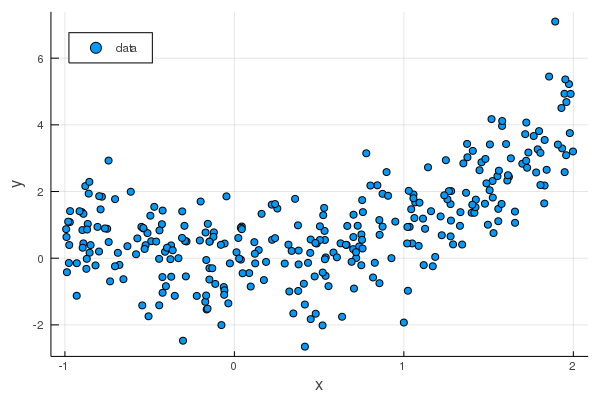
\includegraphics[width=13cm]{Images/TITLE/data}
\centering
\end{figure}

Určit distribuci $p(x)$ není nic těžkého, jelikož jsou tato data na ose x rozděleny rovnoměrně a to přesněji na intervalu $\left(-1 , 2 \right)$. To můžeme určit například z histogramu x-ových souřadnic jednotlivých bodů. 
\begin{equation}
p(x) = \mathrm{U}(-1,2)
\end{equation}
\\Nyní přejdeme k hledání distribuce $p\left(y\vert x \right)$. Tu můžeme určit pomocí metody nejmenších čtverců \eqref{regresethetahat}, protože víme že pro takovou distribuci platí
\begin{equation}
 p(y\vert x) = \pazocal{N}\left(\mathbb{X}\theta, \sigma^2 I \right)
 \end{equation}
kde $\sigma^2$ je rozptyl jedné složky šumu $\varepsilon_i$ a matice $\mathbb{X}$ je ve tvaru definovaném pomocí \eqref{eq:regresematrix}. Nyní máme obě složky k určení $p(y,x)$, zobrazme proto tzv. contour plot, abychom si udělali představu, jak tato distribuce vypadá. 

\begin{figure}[h]
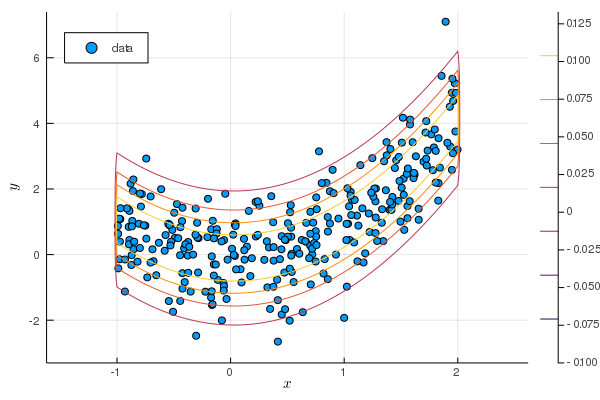
\includegraphics[width=13cm]{Images/TITLE/data_contour}
\centering
\end{figure}

\section{Neuronová síť} 
V sekci \eqref{least_squares} pojednávající o metodě nejmenších čtverců, jsme zmiňovali  pouze lineární funkci \eqref{linear_combination}
\begin{equation}\label{linear_combination}
\hat{y}(x, \theta) = \theta_0 + \theta_1x + \theta_2x^2 + \dots + \theta_px^p = \sum_{i = 0}^{p} {\theta_{i}x^{i}}
\end{equation}
Nyní se pokusíme tento model rozšířit tím, že do něj vneseme nelineární funkci $\phi_j\left(x\right)$
\begin{equation}\label{linear_combination}
\hat{y}(x, \theta) = \sum_{i = 0}^{p} {\theta_{i}x^{i}}
\end{equation}


\section{Variační autoencoder}
Jedna z mnoha metod, jak využít neuronové sítě, je metda variačního autoencoderu. Cílem  je najít hustotu $p(x)$ vzorků $\left\lbrace x_{i} \right\rbrace^N_{i=1} $, jehož empirická hustota se dá zapsat pomocí Diracovy delta funkce
\begin{equation}
p_{\mathrm{emp}}(x) = \frac{1}{N}\sum^N_{i=1}\delta \left(x-x_{i}\right)
\end{equation}
Předpokládáme následující vztahy $x = f_{\theta}(z) + \epsilon$, $\epsilon \sim \pazocal{N}\left(0,\sigma^2I \right)$ a vzájemnou nezávislost $x_{i}$. Z toho můžeme určit distribuce:
 
\begin{equation}
\begin{split}
 p(x\vert z) &= \pazocal{N}\left(f_{\theta}(z),\sigma^2I \right), \\
p(z) &= \pazocal{N}\left(0,I \right),
\end{split}
 \end{equation}
 a proto má smysl využít následující formu apromaximace
\begin{equation}
p(x) = \int p(x\vert z)p(z)\dd z
\end{equation}
\subsection{Naivní přístup}
K nalezení $p(x)$ je třeba najít parametry $\theta$ transformace $f_{\theta}(z)$, proto zkusme využít KL-divergence a  hledat tak $\theta$ minimalizací $D_{KL}\left(p_{\mathrm{emp}}(x) \Vert p_{\theta}(x)  \right)$
\begin{equation}
\begin{split}
\hat{\theta} & = \argmin \sum_{i=1}^n \log p\left(x_{i} \right) \\
& =  \argmin \sum_{i=1}^n \log \int \pazocal{N}\left(f_{\theta}(z),\sigma^2 \right)\pazocal{N}\left(0,1 \right)    \dd z \\
& = \argmin \sum_{i=1}^N \ \log\sum_{j=1}^N \exp \left\lbrace -\frac{1}{2\sigma^2} \left(x - f_{\theta}(z)  \right)^2 \right\rbrace 
\end{split}
\end{equation}
Integrace přes $z$ je nahrazena vzorkováním. Tento postup ovšem nemusí konvergovat ke správným výsledkům.
\subsection{Variační Bayseova metoda}
Lepší metodou se ukazuje vzorkovat z podmíněné distribuce $q(z\vert x)$ a využít ELBO: 

\begin{equation}
\begin{split}
D_{KL}\left(q\left(z\vert x \right) \Vert p(z\vert x)\right) & = 
 \mathbb{E}_q\left[\log q(z\vert x) - \log p\left(z\vert x \right)\right] \\
 & =  \mathbb{E}_q\left[\log q(z\vert x) - \log p(x\vert z) - \log p(z) + \log p(x)   \right]
 \end{split}
\end{equation}
Tuto rovnici můžeme přepsat pomocí KL-divergence 
\begin{equation}
\log p(x) - D_{KL}\left(q\left(z\vert x \right) \Vert p(z\vert x)\right) = \mathbb{E}_q\left[\log p(x\vert z) \right] - D_{KL}\left(q\left(z\vert x \right) \Vert p(z)\right)
\end{equation}
kde pravá strana této rovnice je lower bound $\log p(x)$.
Jestliže vybereme parametrickou formu distribuce
\begin{equation}
q\left(z\vert x \right) = \pazocal{N}\left(\mu_{\phi}(x), \diag\left(\sigma^2_{\phi}(x)\right) \right)
\end{equation}
můžeme parametry $\theta$ a $\phi$ minimalizovat zároveň a to následovně:
\begin{equation}
\begin{split}
\hat{\theta},\hat{\phi} & = \argmin\sum_{i=1}^n\log p\left(x_i\right) \\
& = \argmin\left\lbrace  \mathbb{E}_q\left[\log p(x\vert z) \right] - D_{KL}\left(q\left(z\vert x \right) \Vert p(z)\right)\right\rbrace 
\end{split}
\end{equation}
V metodě variačního autoencoderu jsou důležité následující dvě věci. První je trik v reparametrizaci
\begin{equation}
z = \mu(x) + \sigma(x)\odot\epsilon 
\end{equation}
kde $\odot$ značí Hadamardův součin, čili součin po složkách. Druhý trik je fakt, že KL-divergence dvou gaussovských distribucí má analytické řešení:
\begin{equation}
\begin{split}
 D_{KL}\left(q\left(z\vert x \right) \Vert p(z)\right) & = \frac{1}{2}\left[\tr(\sigma_{\phi}^2(x)) - \mu_{\phi}\tran(x)\mu_{\phi}(x) - k - \log\det \left(\sigma_{\phi}^2(x)   \right)\right] \\
 & = \frac{1}{2}\left[\sum_{l = 1}^k(\sigma_{\phi}^2(x)) -\mu\tran(x)\mu_{\phi}(x) - k - \sum_{l = 1}^k\log\sigma_{\phi}^2(x)    \right]
\end{split}
\end{equation}
Kdybychom totiž nevybrali aproximační distribuci gaussovskou, nemohli bychom tímto způsobem $\hat{\theta},\hat{\phi}$ určit. Toto řešení KL-divergence vede na konečný tvar
\begin{equation}
\hat{\theta},\hat{\phi} = \argmin\left[\sum_{i = 1}^n\sum_{j = 1}^p \left[ x_i - f_\theta \left(\mu_{\phi}(x_i) + \sigma_{\phi}(x_i)\odot\epsilon_{i,j}  \right)        \right] - \frac{1}{2}\left[\sum_{l = 1}^k(\sigma^2_{\phi}(x_i)) -\mu_{\phi}\tran(x_i)\mu_{\phi}(x_i) - k - \sum_{l = 1}^k\log\sigma^2_{\phi}(x_i)   \right] \right]
 \end{equation}
\subsection*{Příklad}

\chapter{Stromové struktury}
Stromovou strukturou dat rozumíme množinu datových záznamů popsaných pomocí množiny vrcholů a hran. Vrcholy dané stromové struktury představují jednotlivé body $x$ a $y$. V podstatě si to můžeme představit opravdu jako strom - má jeden kořen, v první úrovni se dělí na $k_1$ větví, každá další větev se v druhé úrovni dělí na $k_{2_i}$ a tak dále.  My se v této práci budeme zabývat pouze kořenem a první úrovní větví. Ilustrujeme to na jednoduchém příkladu.
\subsection*{Příklad}
Mějme vektor pozorování $\textbf{y} = \left(y_1,\dots,y_n \right)$. Předpokládejme takový model, který ke každému $y_i \in \textbf{y}$, přiřazuje vektor datových záznamů $\textbf{x}_{i}$, $i \in \left\lbrace 1,\dots,n \right\rbrace$, přičemž každý $\textbf{x}_i $ má různý počet prvků $x_j^{(i)}$, $j\in\left\lbrace 1,\dots,k_i \right\rbrace$. Máme tedy $\pazocal{X} = \left(\textbf{x}_1,\dots,\textbf{x}_n \right)$, kde každý vektor $\textbf{x}_i$ může mít jiný počet prvků $k_i$. Celkový počet datových záznamů v $\pazocal{X}$ je $m$, platí tedy $\sum_{i = 1}^{n}\sum_{j = 1}^{k_i} x_j^{(i)} = m$.  Přiřazení probíhá následujícím způsobem:
\begin{equation}
\begin{split}
\textbf{x}_1 & \longmapsto  y_1 \\
\textbf{x}_2 & \longmapsto  y_2\\
\vdots \\
\textbf{x}_n & \longmapsto   y_n
\end{split}
\end{equation}

Jednoduše řečeno je to přiřazení popořadě. Vektor takových $x_j^{(i)} \in \textbf{x}_i$ , přiřazených k jednomu $y_i$ nazveme $\textbf{plukem}$.
Počet prvků v jednom pluku $k_i$ nechť je generován například Poissonovým rozdělením, $k_i \sim  \mathrm{Po}(\lambda)$ a všechny prvky $\pazocal{X}$ nechť jsou například generovány pomocí uniformního rozdělení, $x_j^{(i)} \sim \mathrm{U}(a,b)$.  Jednotlivá $y_i$ potom můžou být určena nějakou závislostí na $\textbf{agregační funkci}$ prvků v plucích k  nim přiřazených. $\textbf{Agregační funkcí}$ budeme rozumět takovou funkci, která dokáže seskupit, nebo-li agregovat, vícero datových záznamů do jednoho. Nejčastěji používané agregační funkce jsou aritmetický průměr, maximum, minimum, nebo součet.    \\
 Pokusme se nalézt sdruženou distribuci $p(y, \bar{\textbf{x}}_{i})$, kde  $\bar{\textbf{x}}_{i}$ značí aritmetický průměr prvků v i-tém pluku
  \begin{equation}
  \bar{\textbf{x}}_{i} = \frac{1}{k_i}\sum_{l = 1}^{k_i} x_l^{(i)} 
 \end{equation}
 
  Použijeme opět součinové pravidlo 
\begin{equation}
p(y, \bar{\textbf{x}}_{i}) = p(y\vert \bar{\textbf{x}}_{i})\cdot p(\bar{\textbf{x}}_{i})
\end{equation}
a pokusme se nalézt tyto dvě distribuce. Tento postup je nám známý už z kapitoly \eqref{generative}. Pro určení podmíněné distribuce $p(y, \bar{\textbf{x}}_{i})$ použijeme opět metodu nejmenších čtverců a dostaneme 
\begin{equation}
p(y, \bar{\textbf{x}}_{i}) = \pazocal{N}\left(\mathbb{X}\theta, \sigma^2 I \right)
\end{equation}
Ovšem zde jsou prvky matice $\mathbb{X}$ jednotlivé prvky z  $\bar{\textbf{x}}_{i}$. Určit distribuci $p(\bar{\textbf{x}}_{i})$ lze určit obdobně pomocí histogramu. Navíc víme-li, že se jedná o výběrové průměry, je z centrální limitní věty jasné, že se bude jednat o normální rozdělení. Střední hodnotu můžeme odhadnout výběrovým průměrem z $\bar{\textbf{x}}_{i}$, tedy
\begin{equation}
 \bar{\bar{\textbf{x}}} = \frac{1}{n}\sum_{i = 1}^n \bar{\textbf{x}}_{i}
\end{equation}
  a rozptyl odhadneme pomocí výběrového rozptylu 
  \begin{equation}
  \Var\left(\bar{\textbf{x}}_{i}\right) = \frac{1}{n}\sum_{i = 1}^n \left( \bar{\textbf{x}}_{i} - \bar{\bar{\textbf{x}}}\right)^2.
\end{equation}  
  
To vede na tvar
\begin{equation}
p(\bar{\textbf{x}}_{i}) = \pazocal{N}\left(\bar{\bar{\textbf{x}}}_{i},\Var\left(\bar{\textbf{x}}_{i}\right) \right)
\end{equation}
Tímto máme spočtené obě složky. Pro vizualizaci sdružené distribuce $p(y, \bar{\textbf{x}}_{i})$ využijeme opět contour plot. 
\begin{figure}[h]
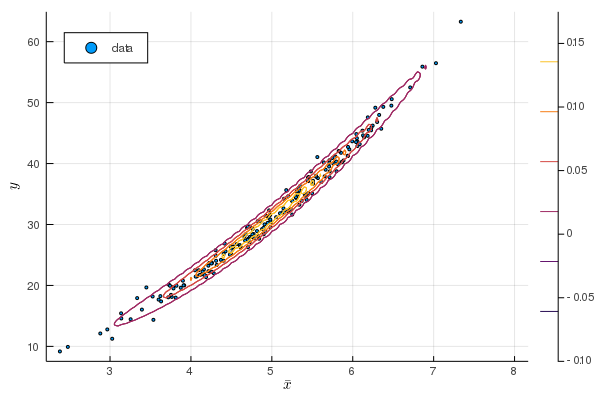
\includegraphics[width=13cm]{Images/TITLE/stromy_joint_distribution_priklad}
\centering
\caption{Countour plot distribuce $p(y, \bar{\textbf{x}}_{i})$, kde $m = 200, \lambda = 10, a = 0, b = 10$ a $y$ závisí na $\bar{\textbf{x}}_{i}$ kvadraticky.}

\end{figure}
Najít distribuci $p(y\vert x)$ není snadný úkol, proto jsme se omezili pouze na hledání distribuce z průměrů jednotlivých složek $\pazocal{X}$.
\chapter*{Závěr}

\pagestyle{plain}

\addcontentsline{toc}{chapter}{Záv\v{e}r}

Text závěru....
\begin{thebibliography}{1}
\bibitem{Allen-Cahn}S. Allen, J. W. Cahn: \emph{A microscopic theory
for antiphase boundary motion and its application to antiphase domain
coarsening}. Acta Metall., 27:1084-1095, 1979.

\bibitem{CINECA}G. Ballabio et al.: \emph{High Performance Systems
User Guide}. High Performance Systems Department, CINECA, Bologna,
2005. \url{www.cineca.it}

\bibitem{rumpf3}J. Becker, T. Preusser, M. Rumpf: \emph{PDE methods
in flow simulation post processing}. Computing and Visualization in
Science, 3(3):159-167, 2000.
\end{thebibliography}

\end{document}
